\section{Implementáció}

\subsection{Fejlesztő környezet}

Mind a kliens, mind a szerver oldal implementálása Java nyelven történik. A kliens oldal az Ericsson Service Development Studio (SDS) 4.1 fejlesztőeszköz segítségével valósult meg. Az SDS az Ericsson honlapján 2010 végéig egy szabadon hozzáférhető fejlesztő környezet volt, jelenleg az alkalmazás támogatása megszűnt, így az le sem tölthető\footnote{Az eszközt, valamint a dokumentációt még korábban, az egyetemi önálló labor keretein belül szereztem be.}. A fejlesztőeszköz képes emulálni az IMS hálózat főbb funkcionális egységeit, így lehetőséget teremt IMS hálózatra szánt alkalmazások fejlesztésére, valamint azok tesztelésére. Az SDS a nyílt forráskódú Eclipse fejlesztői környezetre épül, így az egész rendszer bármilyen, Microsoft Windows XP operációs rendszert futtató PC-n használható. Szabványosított API-kat használhatunk kliens és szerveroldali programozáshoz, valamint a kommunikációs folyamatok, szolgáltatások megvalósításához egyaránt. A fejlesztői keretrendszerbe beépített tesztelési egységek lehetőséget nyújtanak végpontól végpontig tartó tesztelésre. Az SDS tartalmaz előre elkészített funkciókat is, amelyeket a fejlesztők felhasználhatnak az új szolgálatások elkészítése során. Ilyen funkció például a jelenlét, csoport és adatkezelés (Presence, Group and Data Management), amely funkciót az általam fejlesztett csoportos üzenetküldő szolgáltatásban is használok.

\subsubsection{Az SDS IMS maghálózat támogatása}

A fejlesztői PC-n kialakított, SDS által nyújtott IMS emulációs környezet felépítése \aref{fig:sds_env}.~ábrán  látható. Mint ahogy az ábrán is látható, az SDS IMS környezeti emulátorokat (CSCF, DNS, HSS, SIP Proxy), valamint az elkészült szerveroldali alkalmazások futtatásához SIP alkalmazás szervert tartalmaz. Lehetőségünk van saját SIP alkalmazás szervert üzembe állítani, majd az SDS-t úgy konfigurálni, hogy az általunk kívánt alkalmazás szervert használja\footnote{A szerveroldali szolgáltatás futtatásához a BEA Weblogic SIP Server 3.1-es verzióját használtam.}. 

\begin{figure}[htbp]
\center
\resizebox{14cm}{!}{
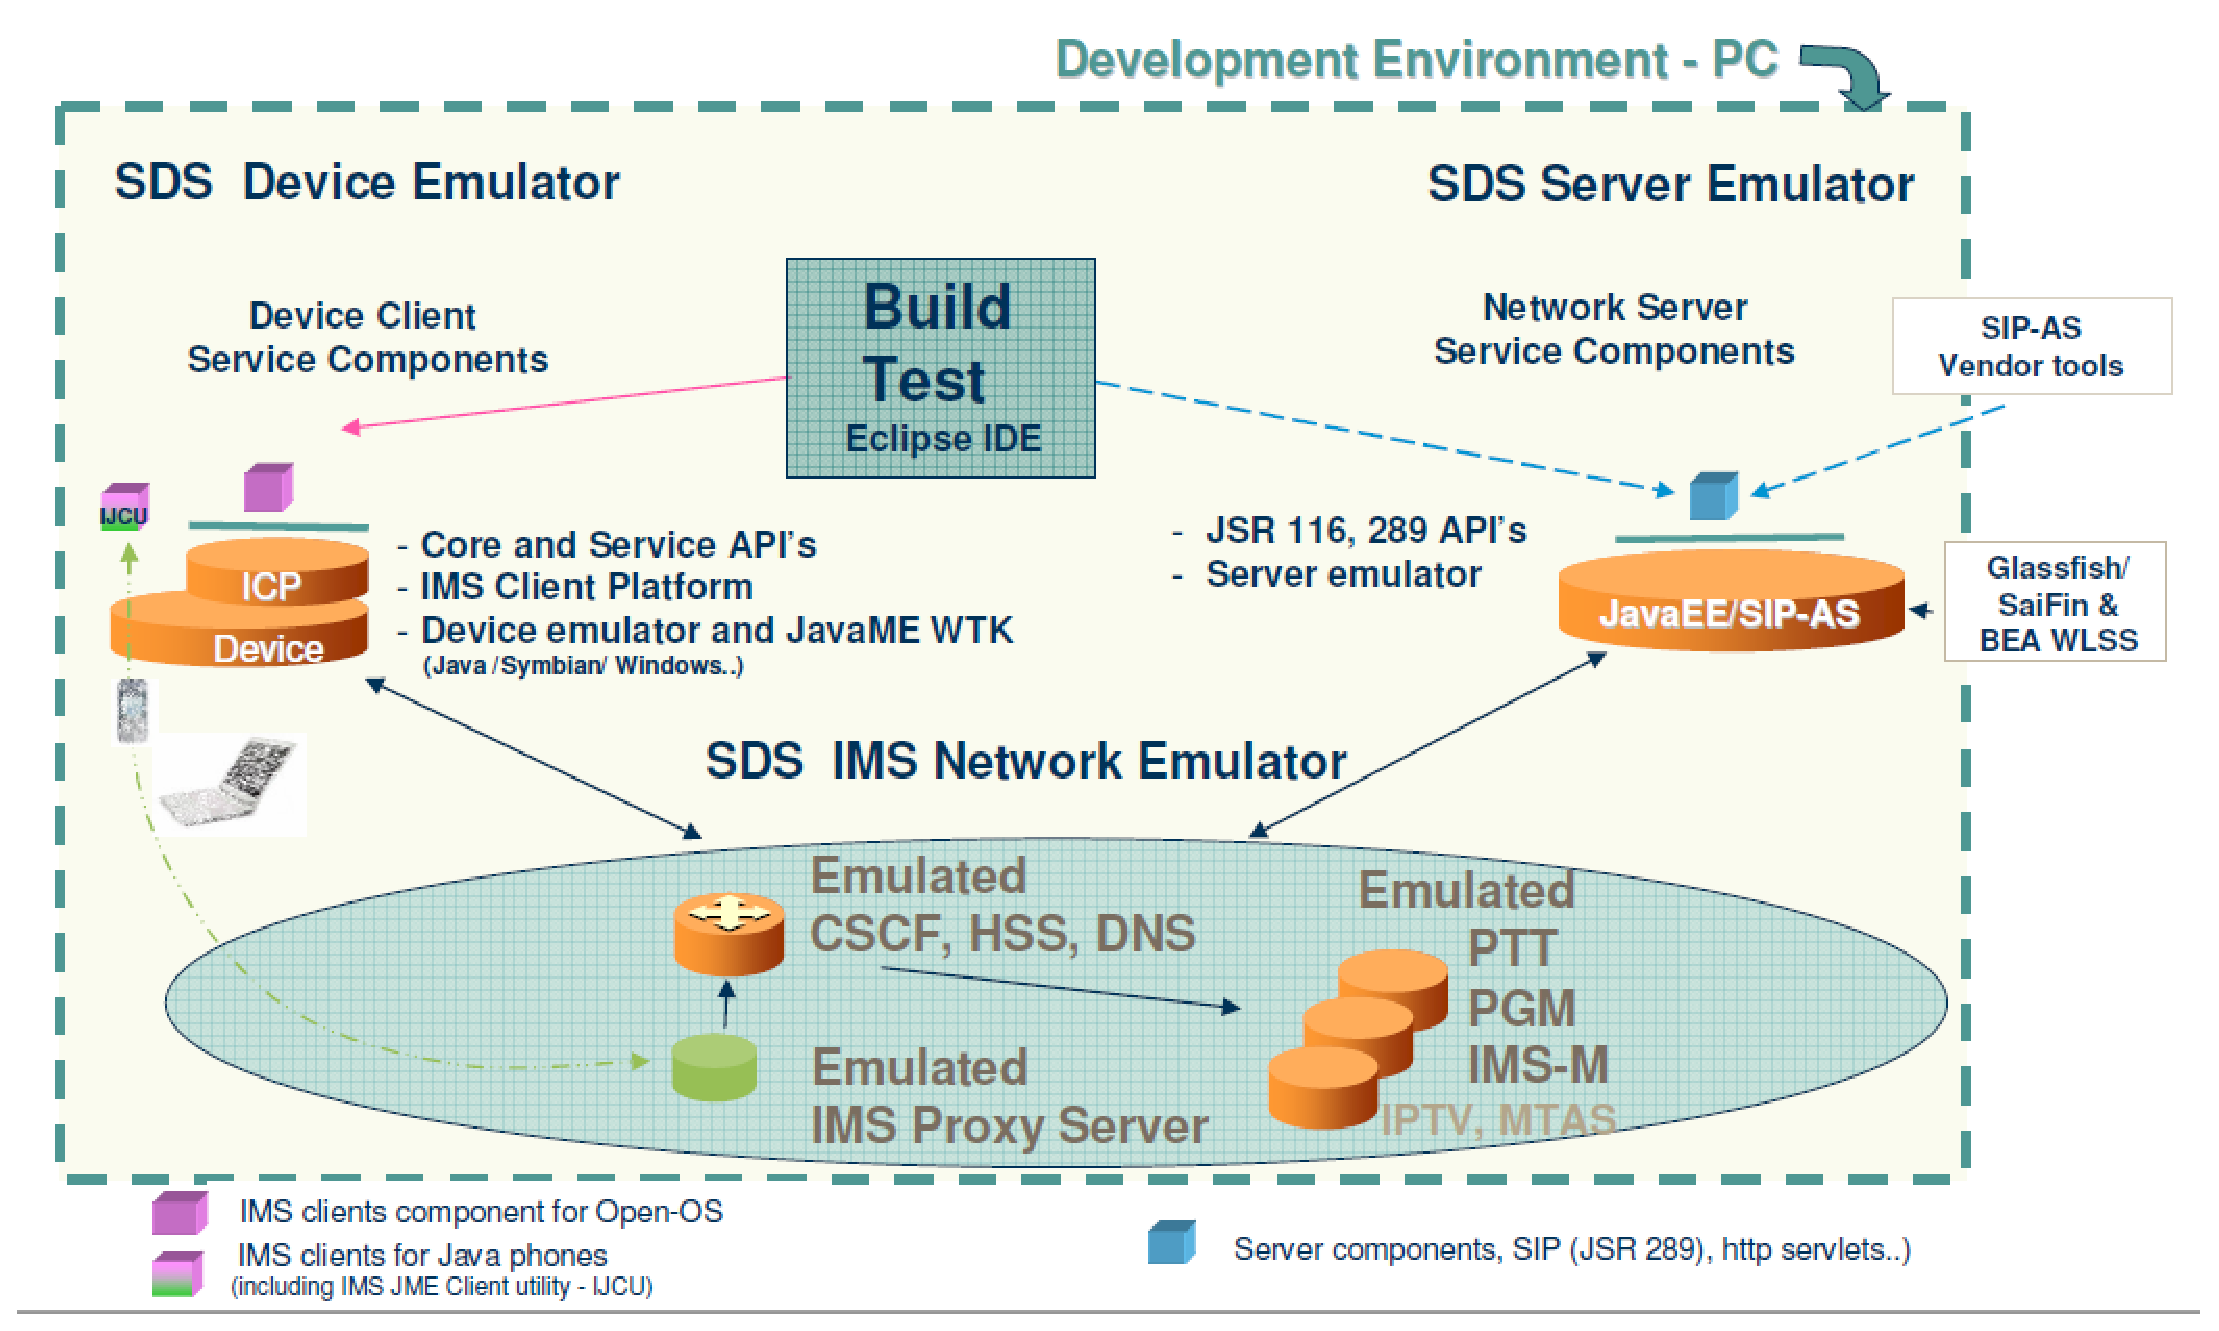
\includegraphics{img/sds-overview.eps}}
\caption{A fejlesztői PC-n kialakított emulációs környezet felépítése}
\label{fig:sds_env}
\end{figure}

Az IMS eszközök legfontosabb beállításait az Eclipse IDE Provisioning nézetében tekinthetjük meg, illetve módosíthatjuk. Itt található a registrar, amely az aktuálisan, CSCF-hez beregisztrált felhasználókat táblázatos formában jeleníti meg. A HSS fül alatt hozhatunk létre felhasználókhoz rendelhető profilokat. Itt hozhatunk létre IFC-ket (Initial Filter Criteria), valamint SPT-ket (Service Tigger Point). Az SPT egy összetett logikai kifejezés, amely a SIP üzenetek bizonyos tulajdonságaira létrehozható logikai állítás. Ilyen logikai állítás lehet a SIP üzenet típusára tett megkötés, vagy a SIP üzenet fejlécére vonatkozó állítás, valamint a request URI-ra tett állítás. Az SPT-t összefoghatóak egyetlen IFC-be, amely tulajdonképpen belépési pont az alkalmazásokhoz. Ilyen módon egyszerűen, logikai állítások halmazával meghatározható, hogy bizonyos feltételek teljesülése esetén mely alkalmazások legyenek értesítve. A létrehozható profilok lényegében IFC-k halmaza. Ezáltal egy felhasználóhoz rendelt profil meghatározza, hogy a felhasználó melyik szolgáltatások használatára jogosult, és melyikre nem. 

\subsubsection{Az SDS kliens oldali készülékek támogatása}

Az SDS kliens oldali fejlesztéshez is nyújt eszközt, amely az IMS Client Framework (ICF) nevet kapta. Az ICF-nek két fő része van. 

Az egyik az IMS Client Platform (ICP), amely Windows vagy Symbian platformra nyújt olyan keretrendszert, amely tartalmazza az alapvető IMS szolgáltatásokat, mint például a SIP session menedzsment, vagy a már \ref{sec:group_messaging}.~fejezetben említett PGM szolgáltatás.

Az ICF keretrendszer másik része az IMS Java Client Utility (IJCU). Az IJCU olyan J2ME-t támogató telefonokhoz szolgáltat API-t, amelyek nem támogatják a SIP protokollt. Az ilyen eszközök előtt az IJCU transparensen elrejti a SIP protokollt, és HTTP üzenetekbe ágyazva küld és fogad SIP csomagokat.


\subsection{Az MSRP protokoll megvalósítása}

Az Interneten nem találtam Java nyelven íródott, az MSRP funkcióit megvalósító, használható fejlesztői könyvtárat, ezért a fejlesztés során szükségesnek tartottam az MSRP alapfunkciókat ellátó osztályok implementálását is. Itt jegyezném meg, hogy az általam létrehozott MSRP implementáció nem valósítja meg \acite{rfc4975}.~irodalomban leírt MSRP RFC szabvály minden funkcióját, csak az MSRP kapcsolaton való üzenetküldéshez szükséges alapfunkciókat. Az általam megvalósított részek követik az MSRP protokoll szabályait\cite{rfc4975}. Ebben a részben a multimédia tartalom hálózaton történő átviteléért felelős MSRP funkciókat megvalósító osztályokat mutatom be.  \Aref{tab:msrp_classes}.~táblázatban az említett osztályokat sorolom fel, kiegészítve a felelősségük, funkciójuk rövid leírásával. Az osztályok részletes leírása a fejezet későbbi szakaszában kerül kifejtésre.

\begin{table}[htb]
\center
\begin{tabular}{|l | p{9cm} |}
\hline
{\bf Az osztály neve} & {\bf Az osztály felelőssége}\\
\hline
\hline
Message & Az MSRP üzenetek kötelező paramétereit tartalmazó osztály\\ \hline
Request & Az MSRP kéréseket reprezentáló osztály\\ \hline
Response & Az MSRP válasz típusú üzenetek adatainak tárolása\\ \hline
CompleteMSRPMessage & A teljes üzenetet reprezentáló osztály, amit az MSRP kapcsolaton kívánunk elküldeni\\ \hline
MSRPStack & Az MSRP funkciók elérése MSRP-n kívüli osztályokból\\ \hline
Connections & Az MSRP kapcsolatokat kiszolgáló TCP kapcsolatok tárolása, kezelése\\ \hline
ReceiverConnection & A TCP kapcsolat, amelyen MSRP csomagokat bájtfolyam formájában fogadunk, feldolgozunk\\ \hline
SenderConnection & Különálló kapcsolat az MSRP csomagok küldésére. Minden MSRP kapcsolathoz tartozik egy példánya\\ \hline
Session & Az MSRP kapcsolatot reprezentáló osztály\\
TransactionManager & Az MSRP csomagok tranzakcionált küldéséért felelős, valamint nyugtázási funkciókat lát el\\ \hline
OutgoingMessageProcessor & Az MSRP kapcsolaton küldött üzenet MSRP kérésekbe való ,,darabolása'', MSRP kérések generálása\\ \hline
IncomingMessageProcessor & Az MSRP kapcsolaton érkező üzenetek feldolgozása, továbbítása a tranzakció menedzser felé\\ \hline
MSRPEvent & Az MSRP kapcsolatban bekövetkezett esemény\\ \hline
MSRPListener & Interfész, az MSRP eseményről való értesítő funkciót lát el\\ \hline
MSRPUtil & Az MSRP üzenet példányok előállítása, üzenet konverziós funkciók\\ \hline
\hline
\end{tabular}
\caption{Az MSRP funkciókat megvalósító osztályok}
\label{tab:msrp_classes}
\end{table}

\subsubsection*{A Message osztály}
\label{sec:msrp_message}

\begin{wrapfigure}{r}{0.45\textwidth}
  \vspace{-15pt}
  \begin{center}
    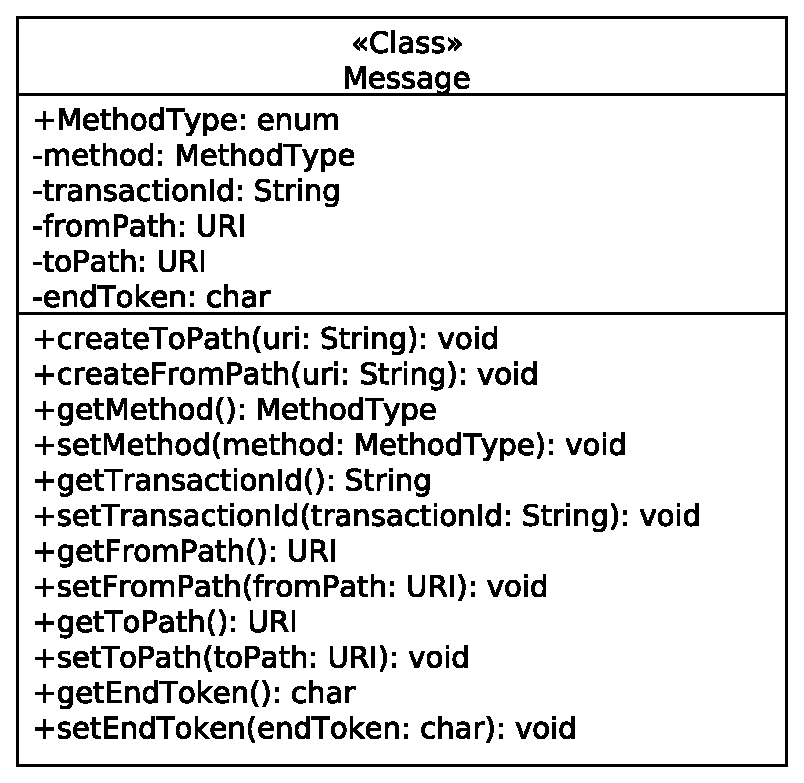
\includegraphics[width=0.43\textwidth]{img/class_diagrams/Message.eps}
  \end{center}
  \vspace{-15pt}
  \captionsetup{font=scriptsize}
  \caption{A Message osztálydiagramja}
   \label{fig:class_message}
  \vspace{-10pt}
\end{wrapfigure}
A Message osztály (\ref{fig:class_message}.~ábra) tartalmazza azokat adatokat, amelyeket minden MSRP csomagban el kell helyezni. Az üzenet típusa -- esetemben kérés (SEND) vagy nyugta (200 OK) -- a method változóban tárolódik. Mivel az MSRP csomagok átvitele tranzakcióban zajlik (küldés -- nyugtázás), így minden csomagnak egyedi tranzakció azonosítója kell, hogy legyen (transactionId). Az MSRP üzenetek fejlécében el kell helyezni az MSRP session lokális és távoli azonosítóját is (toPath, fromPath). Utóbbi két változó értéke a Session osztály remoteURI és localURI változóinak értéke (lásd. \ref{sec:msrp_session}.~pont) kiegészítve az átviteli protokollal (amely minden esetben TCP). Végül eltárolásra kerül az MSRP csomag végét lezáró karakter (\$, +, vagy  \# karakter). A paraméterek módosítására, illetve lekérdezésére metódusok állnak rendelkezésre.

\subsubsection*{A Request osztály}
\label{sec:msrp_request}

\begin{wrapfigure}{r}{0.45\textwidth}
  \vspace{-15pt}
  \begin{center}
    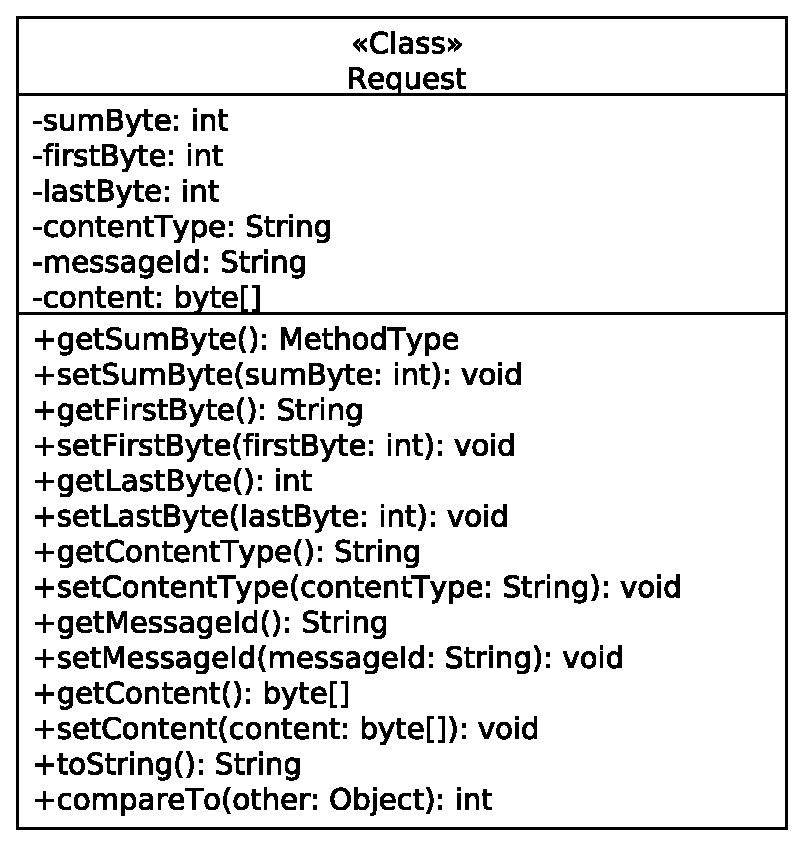
\includegraphics[width=0.43\textwidth]{img/class_diagrams/Request.eps}
  \end{center}
  \vspace{-15pt}
  \captionsetup{font=scriptsize}
  \caption{A Request osztálydiagramja}
   \label{fig:class_request}
  \vspace{-10pt}
\end{wrapfigure}
Az osztály \aref{sec:msrp_message}.~pontban kifejtett Message osztály leszármazottja. A Request osztály reprezentálja az MSRP kapcsolatokon küldött MSRP kéréseket. Az osztály a Message osztályhoz viszonyítva \aref{fig:class_request}.~ábrán látható változókkal, metódusokkal bővül. A sumByte a kérésben átvitelre kerülő teljes MSRP üzenet bájtokban számolt méretét tárolja. Egy teljes MSRP üzenet több kérésben kerül átvitelre, a firstByte és lastByte változók a teljes üzenethez képest az aktuális kérésben átvitelre kerülő első és utolsó bájt sorszámát tárolják. A teljes MSRP üzenet azonosítója a messageId változóba kerül, tehát ugyanazon üzenet más-más darabját ,,hordozó'' MSRP kéréseknek ugyanaz a messageId értéke kell, hogy legyen. A kérés törzsében átvitt adat típusát a contentType mező, míg a tényleges tartalmat a content bájttömb tárolja. 

\subsubsection*{A Response osztály}
\label{sec:msrp_response}

\begin{wrapfigure}{r}{0.45\textwidth}
  \vspace{-15pt}
  \begin{center}
    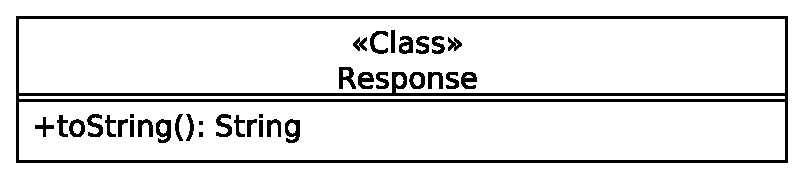
\includegraphics[width=0.43\textwidth]{img/class_diagrams/Response.eps}
  \end{center}
  \vspace{-15pt}
  \captionsetup{font=scriptsize}
  \caption{A Response osztálydiagramja}
   \label{fig:class_response}
  \vspace{-10pt}
\end{wrapfigure}
A Response osztály (\ref{fig:class_response}.~ábra) szintén az Message osztály leszármazottja, így minden paraméterrel és metódussal rendelkezik, ami a Message osztályban szerepel. A Message osztályhoz képest annyiban nyújt többet, hogy felüldefiniálja az osztály toString() metódusát.

\subsubsection*{A CompleteMSRPMessage osztály}
\label{sec:msrp_completmsrpemessage}

\begin{wrapfigure}{r}{0.45\textwidth}
  \vspace{-15pt}
  \begin{center}
    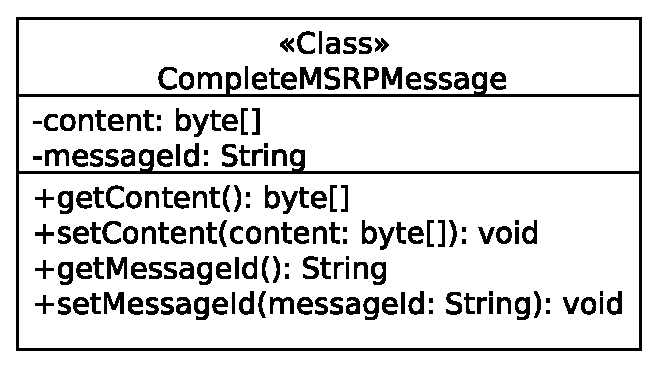
\includegraphics[width=0.43\textwidth]{img/class_diagrams/CompleteMSRPMessage.eps}
  \end{center}
  \vspace{-15pt}
  \captionsetup{font=scriptsize}
  \caption{A CompleteMSRPMessage osztálydiagramja}
   \label{fig:class_completmsrpemessage}
  \vspace{-10pt}
\end{wrapfigure}
A CompleteMessage osztály osztálydiagramja \aref{fig:class_completmsrpemessage}.~ábrán látható. Az osztály tárolja az MSRP kapcsolaton átküldendő üzenet teljes tartalmát (content), illetve az üzenet egyedi azonosítóját (messageId). Az MSRP átvitel során ennek az üzenetnek a tartalmából fognak generálódni \aref{sec:msrp_request}.~pontban tárgyalt MSRP kérés üzenetek. A változók értékeinek lekérdezésére, illetve módosítására metódusok állnak rendelkezésre.

\subsubsection*{Az MSRPStack osztály}
\label{sec:msrp_stack}

\begin{wrapfigure}{r}{0.45\textwidth}
  \vspace{-15pt}
  \begin{center}
    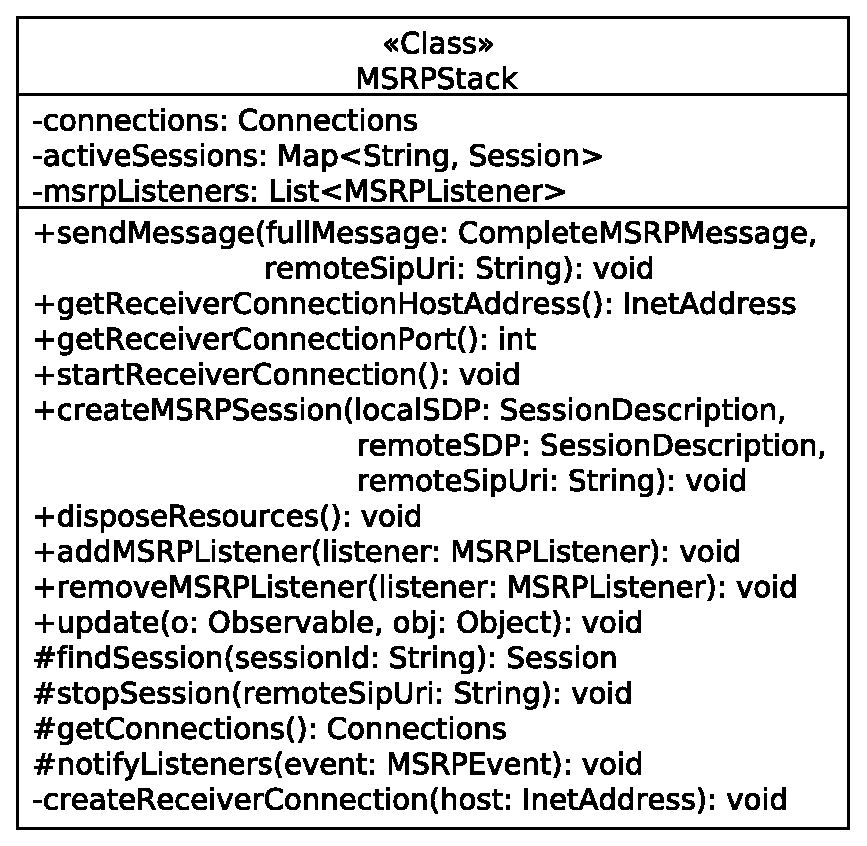
\includegraphics[width=0.43\textwidth]{img/class_diagrams/MSRPStack.eps}
  \end{center}
  \vspace{-15pt}
  \captionsetup{font=scriptsize}
  \caption{Az MSRPStack osztálydiagramja}
  \label{fig:class_msrp_stack}
  \vspace{-10pt}
\end{wrapfigure}
Az MSRPStack osztály (\ref{fig:class_msrp_stack}.~ábra) feladata az MSRP funkciók nyújtása az alkalmazás számára. Az osztály privát változói között szerepel az MSRP kapcsolatokat kiszolgáló TCP kapcsolatokat kezelő osztály (connections), az aktív MSRP kapcsolatokat tartalmazó map (activeSessions), valamint az MSRP eseményekre feliratkozott osztályok listája (msrpListeners). Az activeSessions map a távoli fél egyedi SIP URI-ját használja, mint kulcs attribútum. Az osztály segítségével egy távoli fél felé létrehozhatunk új MSRP kapcsolatot (\mbox{createMSRPSession}). Lekérdezhetünk annak lokális TCP kapcsolatnak az adatait, amelyen keresztül olvashatjuk az aktív MSRP kapcsolatonon beérkező üzeneteket (getReceiverConnectionHostAddress, getReceiverConnectionPort). Ha egy meglévő MSRP kapcsolaton üzenetet kívánunk küldeni, akkor ezt a sendMessage publikus metódus meghívásával tehetjük meg. Az MSRP kapcsolatokat a távoli fél SIP URI-jával azonosítjuk. Egy külső osztály az MSRP eseményekre feliratkozni az addMSRPListener metódussal, míg az eseményekről leiratkozni a removeMSRPListener metódus meghívásával tud. A védett (protected) metódusokat csak az MSRP-t megvalósító osztályok használják.

\subsubsection*{A Connections osztály}
\label{sec:msrp_connections}

\begin{wrapfigure}{r}{0.45\textwidth}
  \vspace{-15pt}
  \begin{center}
    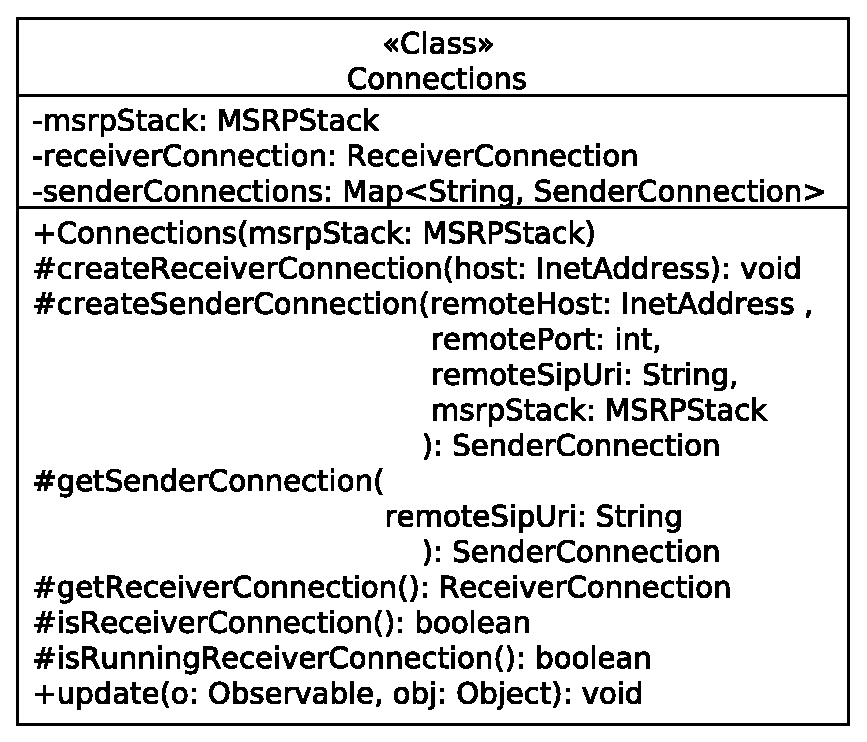
\includegraphics[width=0.43\textwidth]{img/class_diagrams/Connections.eps}
  \end{center}
  \vspace{-15pt}
  \captionsetup{font=scriptsize}
  \caption{A Connections osztálydiagramja}
   \label{fig:class_connections}
  \vspace{-10pt}
\end{wrapfigure}
A Connections osztály felépítése \aref{fig:class_connections}.~ábrán látható. Az osztály felelős az MSRP kapcsolatokat kiszolgáló, a tényleges adatátvitelért felelős TCP kapcsolatok menedzseléséért. Az osztály metódusaival létrehozhatjuk az MSRP kapcsolatokon beérkező csomagok olvasását megvalósító TCP kapcsolatot (\mbox{createReceiverConnection}), valamint az MSRP kapcsolatokon küldött adatok átviteléért felelős TCP kapcsolatokat (\mbox{createSenderConnection}). Mivel az MSRP kapcsolatokon beérkező üzenetek olvasására elegendő egyetlen TCP kapcsolat, így abból csak egy van, ellenben a távoli félnek küldött MSRP csomagok átvitelét megvalósító TCP kapcsolatokkal, amelyekből viszont több. Utóbbiból minden távoli félhez külön TCP kapcsolatot kell létrehozni, amit a senderConnections mapben tárolunk el. A map kulcsa a távoli fél SIP URI-ja. Az osztály implementálja az Observer interfészt, ami arra használatos, hogy a TCP kapcsolatok leállításáról értesüljön a Connections osztályt.

\subsubsection*{A ReceiverConnection osztály}
\label{sec:msrp_receiverconnection}

\begin{wrapfigure}{r}{0.45\textwidth}
  \vspace{-15pt}
  \begin{center}
    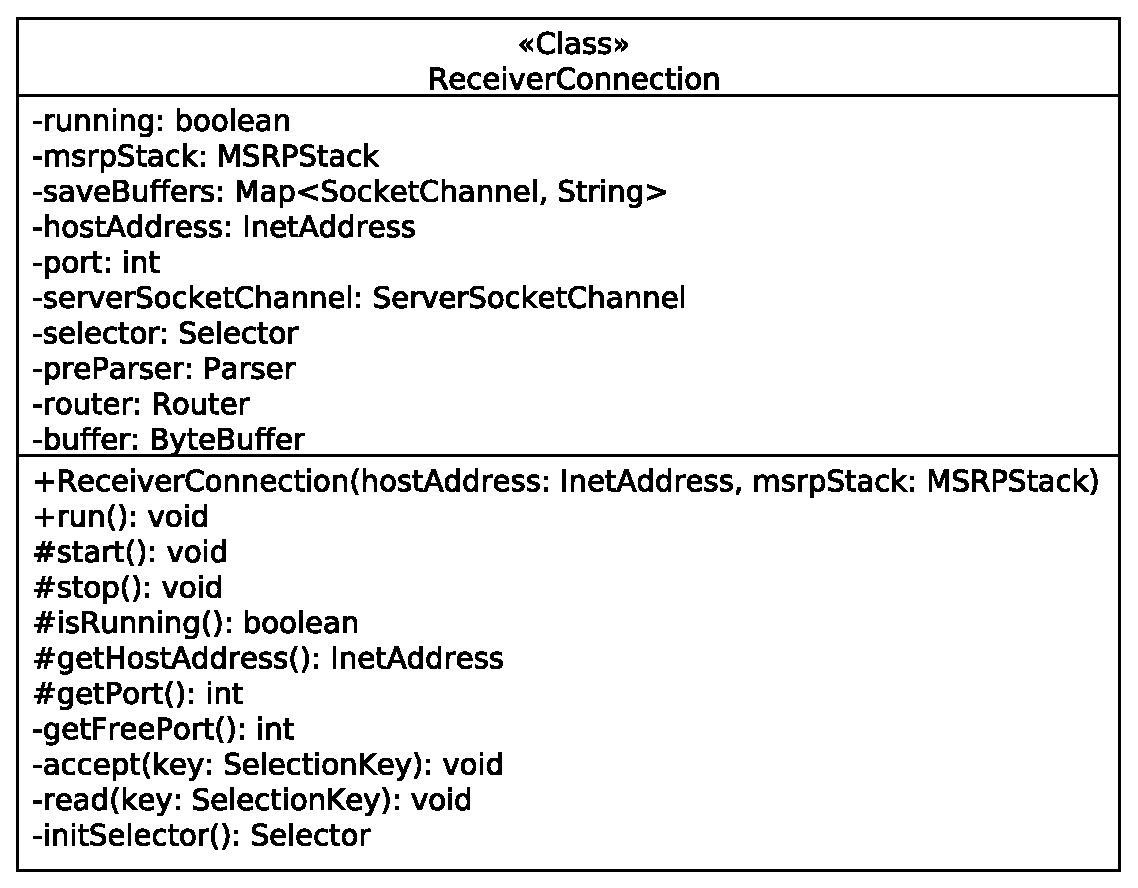
\includegraphics[width=0.43\textwidth]{img/class_diagrams/ReceiverConnection.eps}
  \end{center}
  \vspace{-15pt}
  \captionsetup{font=scriptsize}
  \caption{A ReceiverConnection osztálydiagramja}
   \label{fig:class_receiverconnection}
  \vspace{-10pt}
\end{wrapfigure}
A osztály felépítése \aref{fig:class_receiverconnection}.~ábrán látható. Privát változókban tárolja a kapcsolat állapotát (running), valamint referenciát a kapcsolatot tartalmazó MSRPStack objektumra. Tárolja a TCP kapcsolatok leírását (hoszt cím, port), azok menedzselését (\mbox{serverSocketChannel, selector}) végző objektumokat is. Szintén privát változóban tárolja a TCP kapcsolaton beérkező bájtfolyamból olvasott részadatok átmeneti tárolását végző objektumot (\mbox{saveBuffers}). Két belső osztályt tartalmaz: a Parser, illetve a Router osztályokat. A Parser osztály feladata, hogy a TCP kapcsolaton beérkező bájtfolyamból MSRP csomagokat állítson elő, amelyeknek a további feldolgozását a Router osztály osztály végzi. A Router feladata, hogy az MSRP csomagokat a csomaghoz tartozó MSRP kapcsolathoz eljuttassa. A saveBuffers mapben tárolja a TCP socketből olvasott bájtfolyam végét, azokat az adatokat, amelyek az utolsónak rekonstruált MSRP csomaghoz már nem tartoznak, viszont egy, az adott TCP socket-ből való későbbi olvasás során a következő MSRP csomag részeként használatosak.

\subsubsection*{A SenderConnection osztály}
\label{sec:msrp_senderconnection}

\begin{wrapfigure}{r}{0.45\textwidth}
  \vspace{-15pt}
  \begin{center}
    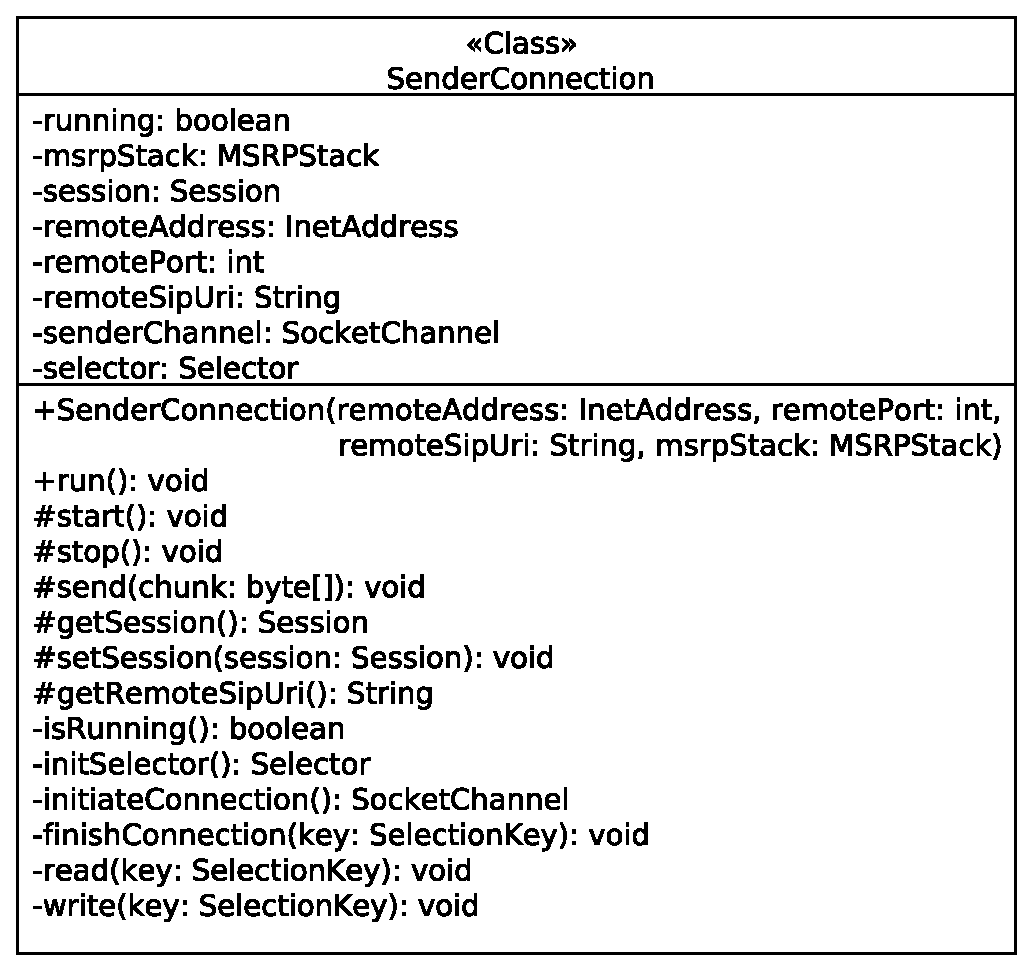
\includegraphics[width=0.43\textwidth]{img/class_diagrams/SenderConnection.eps}
  \end{center}
  \vspace{-15pt}
  \captionsetup{font=scriptsize}
  \caption{A SenderConnection osztálydiagramja}
   \label{fig:class_senderconnection}
  \vspace{-10pt}
\end{wrapfigure}
Az osztály az MSRP kapcsolaton (session), a remoteSipUri változóban tárolt SIP azonosítójú távoli félnek küldött MSRP csomagok továbbítását végzi. Minden különböző SIP URI-val rendelkező kommunikációs partnerhez tartozik egy SenderConnection példány, aminek egyedi azonosítására a remoteSipUri paraméter szolgál. A ReceiverConnection osztályhoz hasonlóan (\ref{sec:msrp_receiverconnection}.~pont) privát változókban tárolja a kapcsolat állapotát (running), referenciát az MSRPStack példányra, valamint a TCP kapcsolatot leíró, illetve vezérlő objektumokat. Az osztály által reprezentált TCP kapcsolaton a kapcsolat sikeres felépítése, valamint elindítása után adatot a send metódus meghívásával tudunk küldeni. A kapcsolat leállítását a stop metódus meghívásával idézhetjük elő.

\subsubsection*{A Session osztály}
\label{sec:msrp_session}

\begin{wrapfigure}{r}{0.45\textwidth}
  \vspace{-15pt}
  \begin{center}
    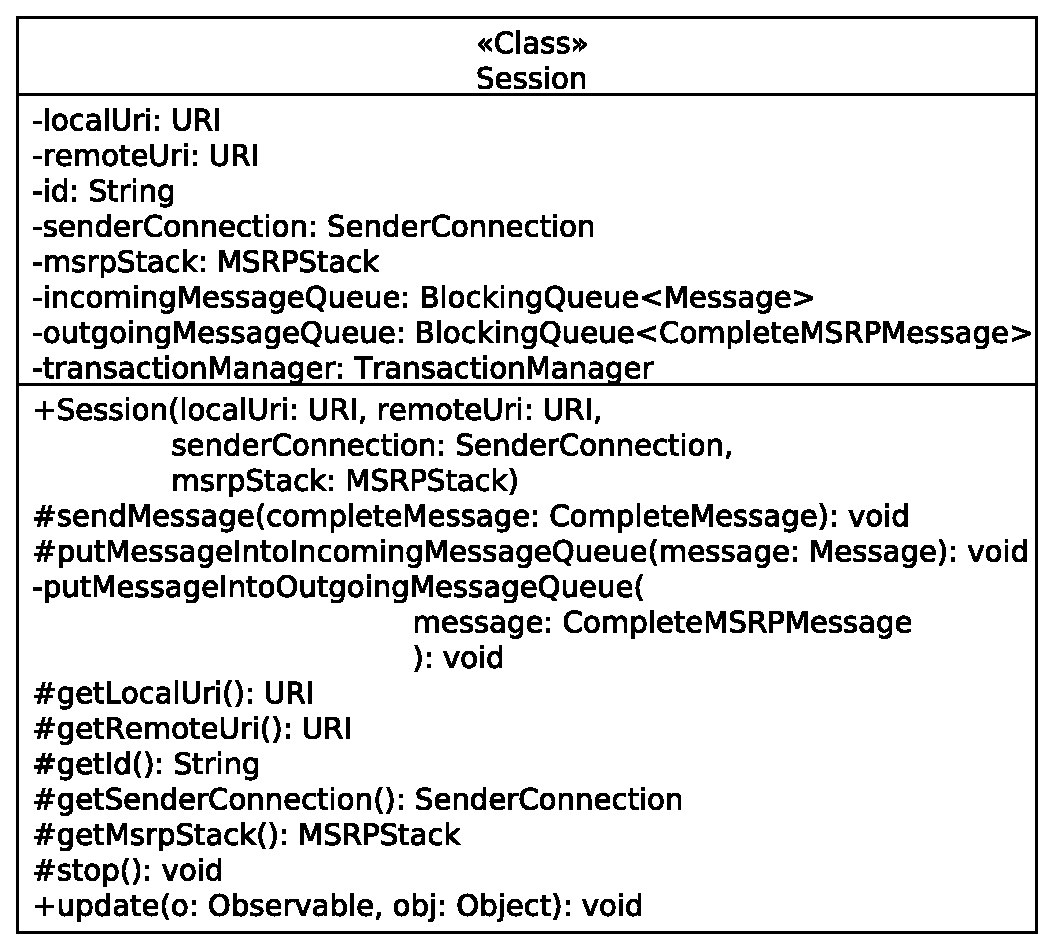
\includegraphics[width=0.43\textwidth]{img/class_diagrams/Session.eps}
  \end{center}
  \vspace{-15pt}
  \captionsetup{font=scriptsize}
  \caption{A Session osztálydiagramja}
   \label{fig:class_session}
  \vspace{-10pt}
\end{wrapfigure}
A Session osztály reprezentálja az MSRP kapcsolatot (\ref{fig:class_session}.~ábra). A localURI és a remoteURI változókban tárolódik a kapcsolatban résztvevő felek MSRP azonosítója. A senderConnection változóban a session-hoz tartozó küldő TCP kapcsolatra referencia tárolódik. Az incomingMessageQueue sorba kerülnek a session-hoz tartozó bejövő MSRP csomagok, míg az outgoingMessageQueue sorba az adott MSRP session-ön küldendő MSRP üzenetek kerülnek. A sorokból a session-t kezelő TransactionManager osztálypéldány részeként az IncomingMessageProcessor, illetve az OutgoingMessageProcessor példányok dolgoznak. A TransactionManager osztály végzi az MSRP kérések tranzakcionált kezelését, azaz a kérések küldését, valamint a bejövő kérések nyugtázását. Az osztály, valamint a két processzor osztály leírása később, \aref{sec:msrp_transactionmanager}., \aref{sec:msrp_incomingprocessor}., valamint \aref{sec:msrp_outgoingprocessor}.~pontokban kerül kifejtésre. Az id változó a session azonosítására szolgál, értéke a két URI konkatenációja. Utóbbi változó az MSRPStack osztályban lévő activeSessions mapben a kulcs attribútum. A stop metódus meghívásával a session példányhoz kapcsolódó minden erőforrás felszabadításra kerül. 

\subsubsection*{A TransactionManager osztály}
\label{sec:msrp_transactionmanager}

\begin{wrapfigure}{r}{0.45\textwidth}
  \vspace{-25pt}
  \begin{center}
    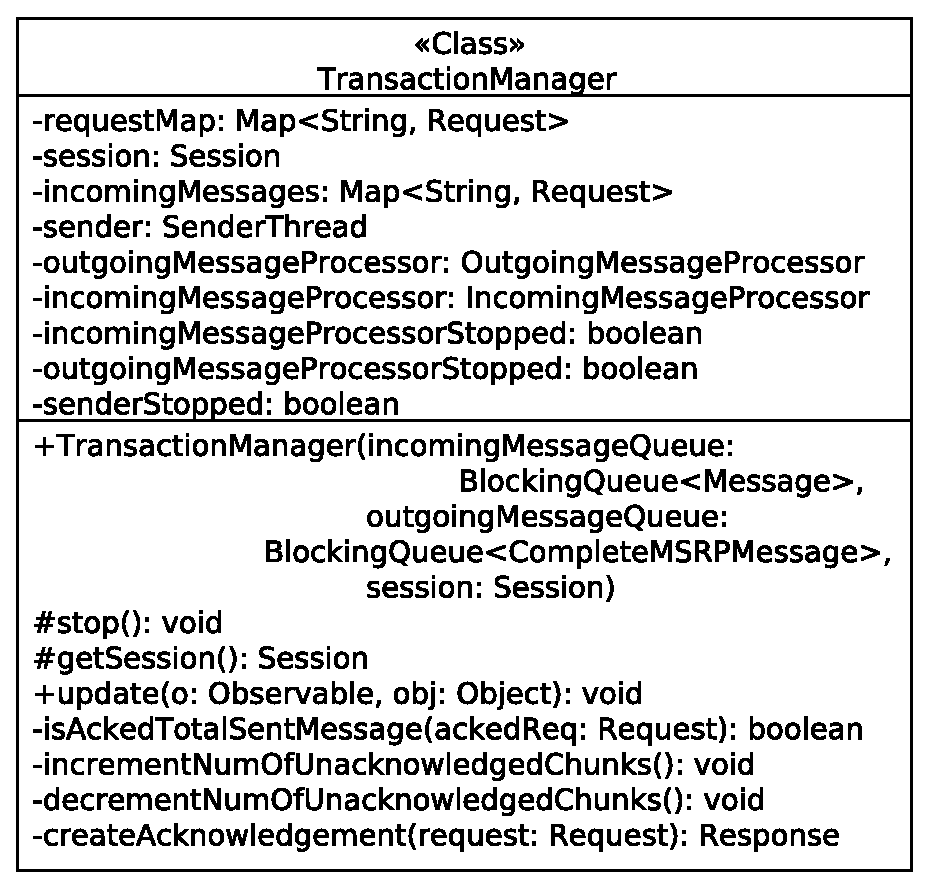
\includegraphics[width=0.43\textwidth]{img/class_diagrams/TransactionManager.eps}
  \end{center}
  \vspace{-15pt}
  \captionsetup{font=scriptsize}
  \caption{A TransactionManager osztálydiagramja}
   \label{fig:class_transactionmanager}
  \vspace{-10pt}
\end{wrapfigure}
A TransactionManager osztály (\ref{fig:class_transactionmanager}.~ábra) minden példánya egy-egy MSRP Session példányhoz (session) tartozik. Az MSRP kapcsolaton bejövő üzeneteket az incomingMessageProcessor példány továbbítja a TransactionManager példánynak. Hasonlóan, az MSRP kapcsolaton kiküldésre szánt üzenetet az outgoingMessageProcessor példány dolgozza fel, azaz teljes üzenetből MSRP kéréseket hoz létre, majd a kéréseket továbbítja a TransactionManager osztálynak, amely a tényleges küldéseket felügyeli. Az osztály a kiküldendő kéréseket egy mapben tárolja (requestMap), amelynek kulcsa az adott MSRP kérés tranzakció azonosítója. Amikor a kérésre nyugta érkezik (amit szintén megkap a TransactionManager), a nyugtához tartozó kérés törlődik az adott map-ből. A TransactionManager ezáltal tartja számon, hogy melyik kérésre nem érkezett még nyugta a távoli féltől. Az osztály másik feladata beérkező MSRP kérések nyugtázása. A beérkező kéréseket az incomingMessages mapben tárolódnak el. Miután az üzenethez tartozó utolsó MSRP kérés is megérkezett, a TransactionManager létrehoz egy MSRP eseményt, majd az MSRPStack példány notifyListeners metódusának meghívásával értesíti erről az aktuális MSRP kapcsolat eseményeire feliratkozott figyelőket.

\subsubsection*{Az OutgoingMessageProcessor osztály}
\label{sec:msrp_outgoingprocessor}
\begin{wrapfigure}{r}{0.45\textwidth}
  \vspace{-15pt}
  \begin{center}
    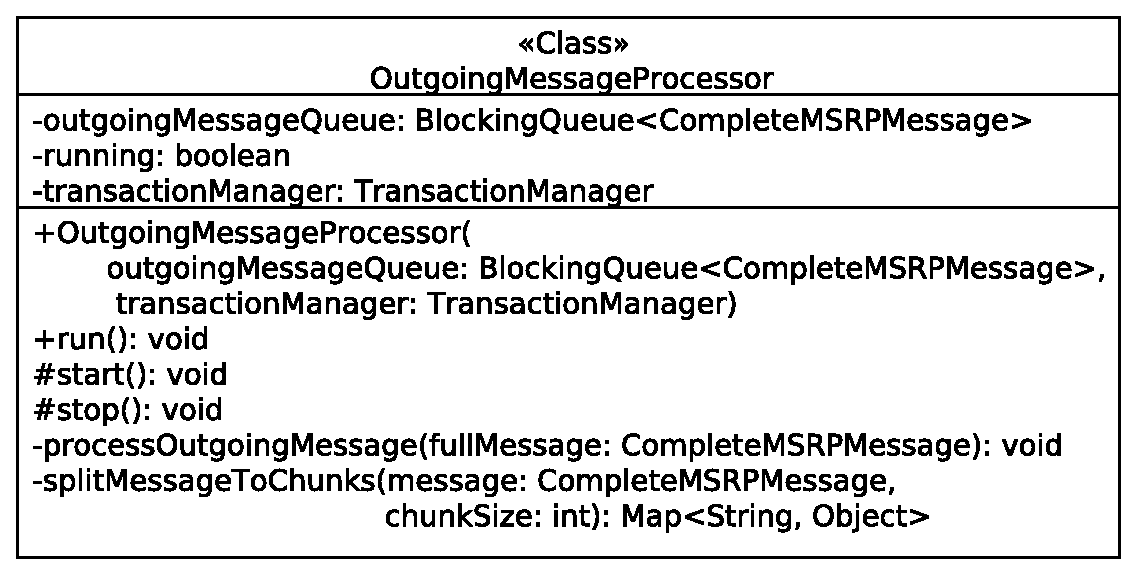
\includegraphics[width=0.43\textwidth]{img/class_diagrams/OutgoingMessageProcessor.eps}
  \end{center}
  \vspace{-15pt}
  \captionsetup{font=scriptsize}
  \caption{Az OutgoingMessageProcessor osztálydiagramja}
   \label{fig:class_outgoingprocessor}
  \vspace{-10pt}
\end{wrapfigure}
Az OutgoingMessageProcessor osztály osztálydiagramja \aref{fig:class_outgoingprocessor}.~ábrán látható. Feladata egyszerű, az MSRP kapcsolaton átvitelre szánt üzeneteket (CompleteMSRPMessage példányokat) kiolvassa a feldolgozási sorból (outgoingMessageQueue), azt meghatározott méretű darabokra tördeli (splitMessageToChunks), majd az egyes darabokból MSRP kéréseket generál, kitöltve a kérésekben szükséges paraméteket. A sikeres feldolgozás után a kérések listáját továbbítja a processzorhoz tartozó tranzakció menedzsernek (transactionManager változó). Start és stop metódusok hívásával indítható, illetve leállítható a processzor működése. 

\subsubsection*{Az IncomingMessageProcessor osztály}
\label{sec:msrp_incomingprocessor}
\begin{wrapfigure}{r}{0.45\textwidth}
  \vspace{-15pt}
  \begin{center}
    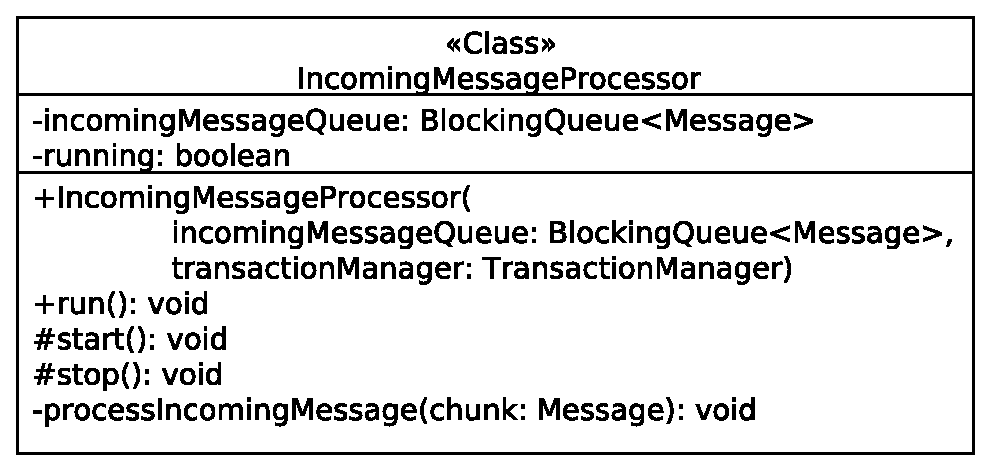
\includegraphics[width=0.43\textwidth]{img/class_diagrams/IncomingMessageProcessor.eps}
  \end{center}
  \vspace{-15pt}
  \captionsetup{font=scriptsize}
  \caption{Az OutgoingMessageProcessor osztálydiagramja}
   \label{fig:class_incomingprocessor}
  \vspace{-10pt}
\end{wrapfigure}
Az IncomingMessageProcessor osztály (\aref{fig:class_incomingprocessor}.~ábra) az MSRP kapcsolaton beérkező üzeneteket dolgozza fel. Az üzeneteket sorból olvassa (incomingMessageQueue), majd attól függően, hogy az MSRP üzenet kérés, vagy válasz, konvertálás után továbbítja azokat a processzort tartalmazó tranzakció menedzser példánynak. 

\subsubsection*{Az MSRPEvent osztály}
\label{sec:msrp_event}

\begin{wrapfigure}{r}{0.45\textwidth}
  \vspace{-15pt}
  \begin{center}
    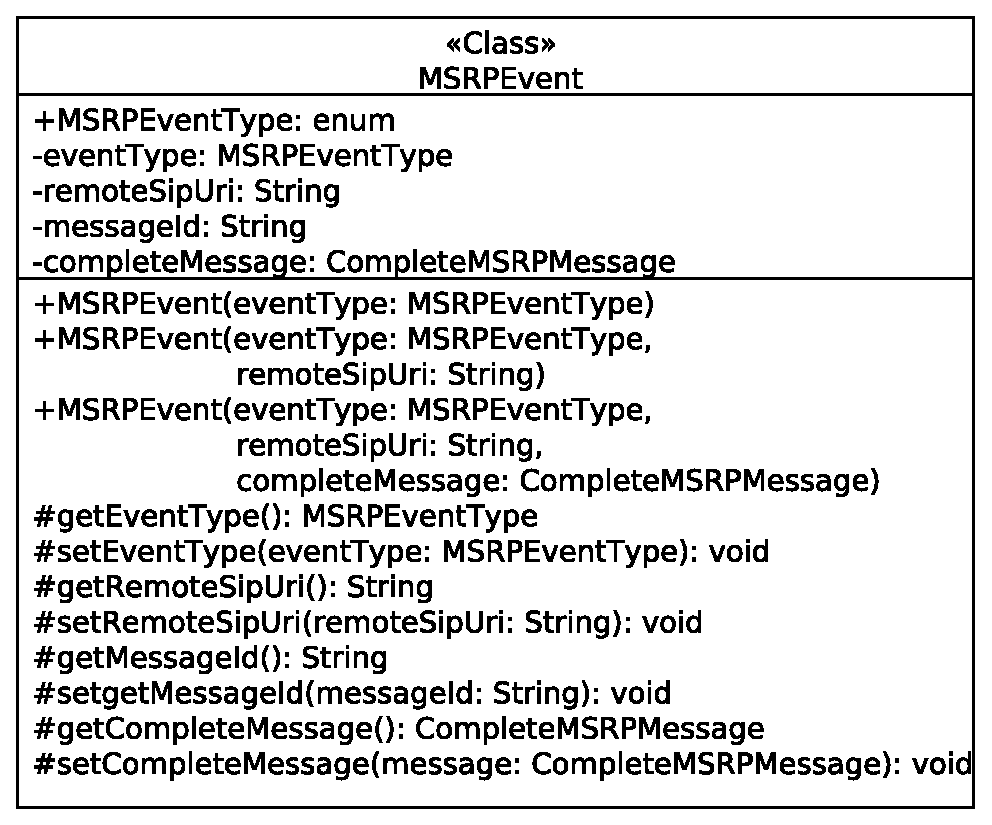
\includegraphics[width=0.43\textwidth]{img/class_diagrams/MSRPEvent.eps}
  \end{center}
  \vspace{-15pt}
  \captionsetup{font=scriptsize}
  \caption{Az MSRPEvent osztálydiagramja}
   \label{fig:class_event}
  \vspace{-10pt}
\end{wrapfigure}
Az MSRPEvent osztály reprezentálja az MSRP kapcsolatokban bekövetkezett eseményeket. Osztálydiagramja \aref{fig:class_event}.~ábrán tekinthető meg. A kapcsolatban bekövetkezett lehetséges események típusát az MSRPEventType felsorolás típus adja meg. Ilyen esemény típus lehet például egy MSRP kapcsolat sikeres létrehozása, vagy egy üzenet összes darabjának sikeres megérkezése, az MSRP kapcsolat megszakadása, stb. Privát változóban tárolja az MSRP kapcsolatban résztvevő távoli fél SIP azonosítóját (remoteSipUri). Opcionálisan megadható az üzenet azonosítója, amely üzenet átvitele során az esemény bekövetkezett. Az eseményben megadható maga, az MSRP kapcsolaton átvitelre került üzenet is (completeMessage), így az egyszerűen továbbítható azoknak az osztályoknak, akik feliratkoztak az eseményekre.

\subsubsection*{Az MSRPListener interfész}
\label{sec:msrp_listener}

\begin{wrapfigure}{r}{0.45\textwidth}
  \vspace{-15pt}
  \begin{center}
    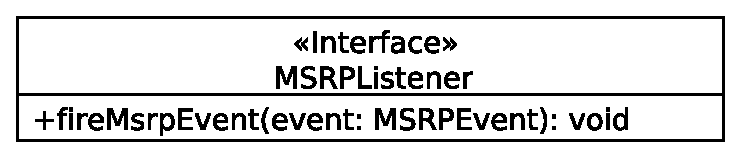
\includegraphics[width=0.43\textwidth]{img/class_diagrams/MSRPListener.eps}
  \end{center}
  \vspace{-15pt}
  \captionsetup{font=scriptsize}
  \caption{Az MSRPListener osztálydiagramja}
   \label{fig:class_listener}
  \vspace{-10pt}
\end{wrapfigure}
Az MSRPListener egy egyszerű interfész (\ref{fig:class_listener}.~ábra), amelynek fireMSRPEvent függvényének implementálásával az implementáló osztály az MSRP kapcsolatokban bekövetkezett eseményekről értesülhet. Ehhez annyit kell tenni, hogy az implementáló osztályt hozzá kell adni az MSRPStack osztály msrpListeners listájához (lásd.:\ref{sec:msrp_stack}.~pont)

\subsubsection*{Az MSRPUtil osztály}
\label{sec:msrp_util}

\begin{wrapfigure}{r}{0.45\textwidth}
  \vspace{-15pt}
  \begin{center}
    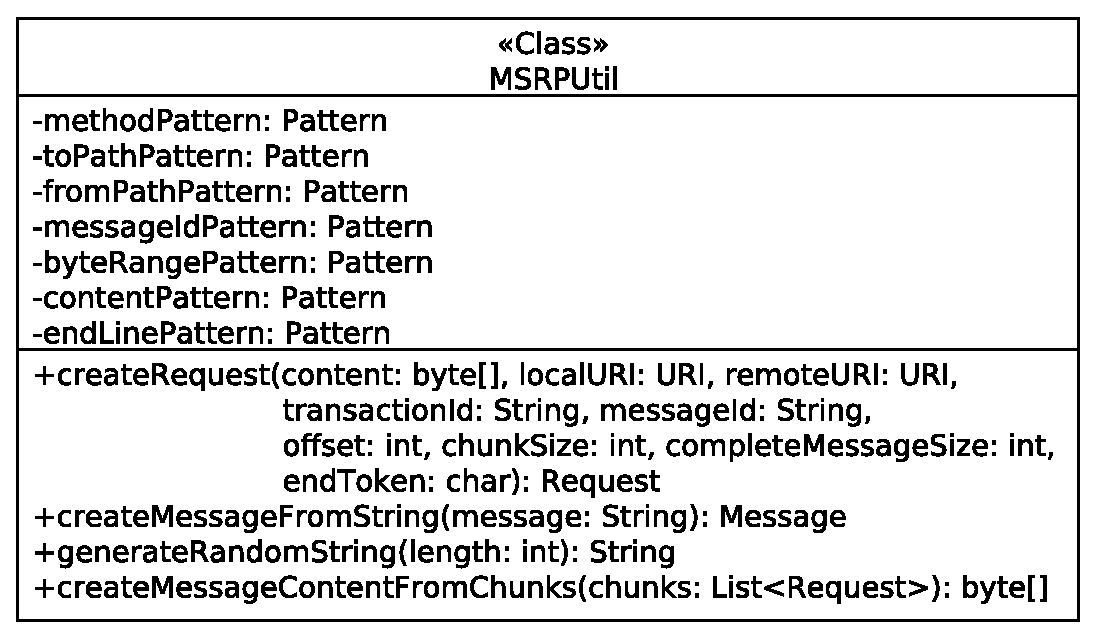
\includegraphics[width=0.43\textwidth]{img/class_diagrams/MSRPUtil.eps}
  \end{center}
  \vspace{-15pt}
  \captionsetup{font=scriptsize}
  \caption{Az MSRPUtil osztálydiagramja}
   \label{fig:class_util}
  \vspace{-10pt}
\end{wrapfigure}
Az MSRPUtil osztály (\ref{fig:class_util}.~ábra) négy statikus segédfüggvényt kínál az MSRP funkciókat megvalósító osztályoknak. A createRequest metódus segítségével a metódusnak paraméterben átadott adatokból egy MSRP kérést (Request) állít elő. A createMessageFromString metódus segítségével egy MSRP üzenet (Message) példányt hozhatunk létre. Az átadott String objektumban bizonyos mintákat keresünk, majd a talált minták alapján létrehozzuk az MSRP üzenetet. A generateRandomString egy adott hosszú véletlen karaktersorozatot ad vissza. A metódus a különböző azonosítók (üzenet azonosító, tranzakció azonosító, MSRP kapcsolat azonosító, stb.) generálására használatos. Végül a createMessageContentFromChunks metódussal a paraméterül átadott MSRP kérésekből visszaállítja az eredeti, MSRP kapcsolaton továbbított üzenetet.